\section{Overview}
\label{sec:overview}

We begin with an overview of \toolname's neurosymbolic
approach to repairing parse errors.
%
Our approach is based on two key insights.
%
\emph{Symbolic} approaches like Error Correcting
Earley (ECE) Parsers \citep{Aho_1972} can, in principle,
synthesize repairs, but, in practice, are overwhelmed by
the many error-correction rules that are irrelevant to the
particular program that requires repair.
%
In contrast, \emph{Neural} approaches
are fooled by the large space of possible
token-sequence level edits, but can precisely
pinpoint the set of EC-rules that are relevant
to a particular program.
%
Thus, \toolname addresses the problem of parse
error repair by a neurosymbolic approach that
combines the complementary methods as summarized
in Figure~\ref{fig:overall-approach}.
%
%
\emph{(Neural component)}
%
Given a dataset of ill-parsed programs and
their fixes, we partially parse the programs
into \emph{abstract sequences} of tokens
(\S~\ref{sec:overview:abstraction}), that can
be used to train \emph{transformer classifiers}
(\S~\ref{sec:overview:train}), that predict
program-relevant error rules for new erroneous
programs (\S~\ref{sec:overview:seq-classifiers})
%
\emph{(Symbolic component)}
%
Next, given an erroneous program, and a (small) set of
predicted \emph{program relevant} error rules, the
the ECE-parser can exploit the high-level grammatical
structure of the language to make short work of
synthesizing the best repair (\S~\ref{sec:overview:ec-parsing}).
%
Next, we give an overview of \toolname, by describing these elements in turn.

%  to repair a program with parse errors. In
% the remainder of this section, we give a high-level overview of our approach
% (presented in \autoref{fig:overall-approach}) by describing how to:

% \begin{enumerate}

%   \item Use an \emph{ECE-Parser} to repair programs with parse errors
%   (\S~\ref{sec:overview:ec-parsing}),

%   \item Abstract erroneous programs with their \emph{partial parses}
%         and the use of Probabilistic Context-Free Grammars (PCFGs)
%         (\S~\ref{sec:overview:abstraction}),

%   \item Train \emph{sequence classifiers} on the abstracted programs
%         to predict subsets of error rules (\S~\ref{sec:overview:train}),

%   \item and \emph{Predict error rules} for new erroneous programs to
%   suggest fixes (\S~\ref{sec:overview:seq-classifiers}).

% \end{enumerate}

\begin{figure}[t]
  \centering
  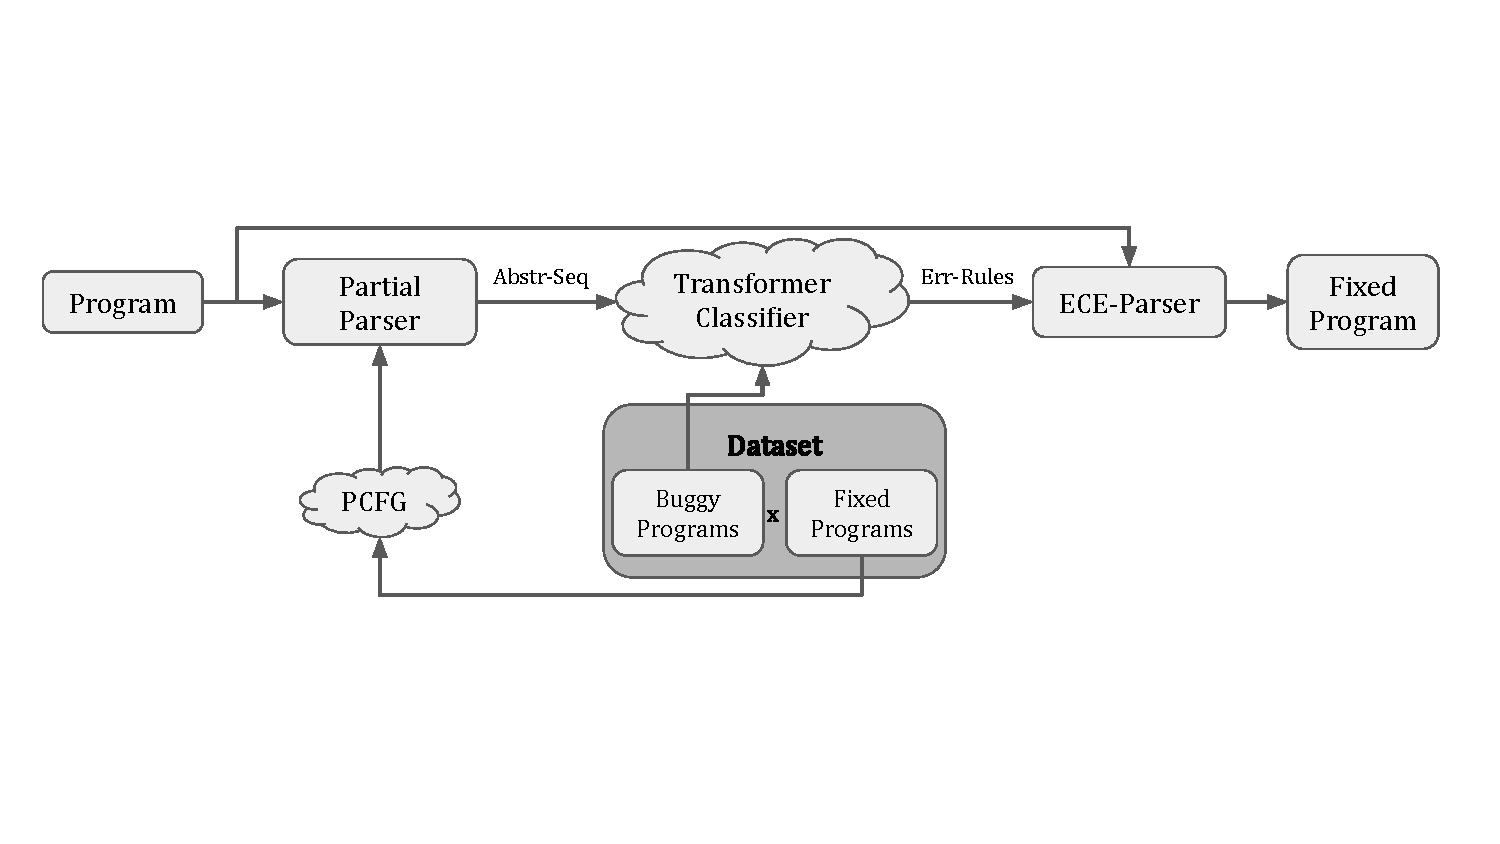
\includegraphics[trim={0 3.8cm 0 3.8cm}, clip, width=0.9\linewidth]{overall-approach.pdf}
  \caption{\toolname's overall approach.}
  \label{fig:overall-approach}
\end{figure}

% \mypara{Error Correcting Parsers}
% One approach to fixing erroneous programs (as in \autoref{fig:bad-prog})
% is to use \emph{Error Correcting Parsers} (EC-Parsers) \citep{Aho_1972}.
% EC-Parsers are based on dynamic programming algorithms and have been used
% to automatically infer the intended parse trees for programs
% that have syntax errors. These dynamic programming parsers have been used
% with \emph{error correcting production rules} \citep{Aho_1972} to
% generate a valid parse by making minimal edits to the original program.
% However, EC-Parsers are very inefficient for larger
% grammars, since they require the addition of a large number of error production
% rules, making them impractical for real-world applications. In contrast, the
% original Earley parsing algorithm is also based on dynamic programming
% but does not directly support error correction~\citep{Earley_1970}.


\begin{figure}[t]
\begin{minipage}[c]{0.47\linewidth}
\begin{rules}
S        $\rightarrow$ Stmts end_marker
Stmts    $\rightarrow$ Stmt \n | Stmt \n Stmts
Stmt     $\rightarrow$ FuncDef | ExprStmt
          | RetStmt | PassStmt | ...
FuncDef  $\rightarrow$ def name Params : Block
Block    $\rightarrow$ \n indent Stmts dedent
RetStmt  $\rightarrow$ return | return Args
Args     $\rightarrow$ ExprStmt | ExprStmt , Args
ExprStmt $\rightarrow$ ArExpr | ...
ArExpr   $\rightarrow$ Literal
          | ArExpr BinOp Literal
Literal  $\rightarrow$ name | number | ...
\end{rules}
\caption{Simplified Python production rules.}
\label{fig:production-rules}
\end{minipage}
\hspace{0.02\linewidth}%
\begin{minipage}[c]{0.50\linewidth}
\hspace*{-0.06\linewidth}%
\begin{figure}
    \centering
    \begin{tikzpicture}
    [font=\small, edge from parent,
    every node/.style={top color=white, bottom color=black!15,
    circle, minimum size=11mm, draw=black!75,
    thick, drop shadow, align=center},
    edge from parent/.style={draw=black!75,thick},
    level distance=1.6cm, xscale=1.3]
    \node (func) {Funcdef}
        child {
            node (def) {\texttt{\bfseries def}}
        }
        child {
            node (name1) {\texttt{Name}}
        }
        child {
            node (params) {\texttt{Params}}
            child {
                node (openParen) {\texttt{\bfseries (}}
            }
            child {
                node (name2) {\texttt{Name}}
            }
            child {
                node (closeParen) {\texttt{\bfseries )}}
            }
        }
        child {
            node (colon) {\texttt{\bfseries :}}
        }
        child [level distance=0.3cm, xscale=1.35] {
            node  (suite) {\texttt{Suite}}
            child [level distance=1.3cm] {
                node (etc) {\texttt{...}}
            }
            child [level distance=1.3cm] {
                node (RetStmt) {\texttt{RetStmt}}
                % node (RetStmt) {\texttt{\begin{tabular}{c}
                %                                 Return\\
                %                                 Stmt
                %                             \end{tabular}}}
                child {
                    node (return) {\texttt{\bfseries return}}
                }
                child {
                    node (ArgList) {\texttt{ArgList}}
                    child [level distance=1.6cm] {
                        node (ArExpr1) {\texttt{ArExpr}}
                        child [level distance=1.3cm] {
                            node (ArExpr2) {\texttt{Literal}}
                        }
                        child [level distance=1.3cm] {
                            node (plus) {\texttt{\bfseries +}}
                        }
                    }
                }
            }
        };
    \end{tikzpicture}
    \caption{The partial parse tree generated for the example at \autoref{fig:orig-prog}}
    \label{fig:partial-parse-tree}
\end{figure}

\end{minipage}
\end{figure}

\subsection{Error Correcting Parsing}
\label{sec:overview:ec-parsing}

\mypara{Earley Parsers for Python}
%
An Earley parser accepts programs that belong to a
language that is defined by a given \emph{grammar} $G$
by using dynamic programming, to store top-down partial
parses in a data structure called a \emph{chart} \citep{Earley_1970}.
The grammar $G$ has a starting symbol |S| and a set of \emph{production rules}.
\autoref{fig:production-rules} presents some simplified production rules for the
Python programming language that will help parse the program in
\autoref{fig:bad-prog}. \emph{Terminal} symbols (or \emph{tokens}) are
syntactical symbols and are here presented in lowercase
letters. Uppercase letters denote \emph{non-terminal} symbols, which are
rewritten using production rules during a parse.
For example, the non-terminal |Stmt| defines all
possible Python statements, including expressions (|ExprStmt|), return statements
(|RetStmt|), \etc \autoref{fig:partial-parse-tree-1} shows the top levels of
the parse tree for the |bar| function in \autoref{fig:bad-prog} using these
productions rules.

%
% \begin{figure}[t]
% \begin{ecode}
% New_S     (*@$$\rightarrow$@*) S | S Insert
% ...
% Block     (*@$$\rightarrow$@*) E_\n E_indent Stmts E_dedent
% RetStmt   (*@$$\rightarrow$@*) ... | E_return | E_return Args
% ...
% E_return  (*@$$\rightarrow$@*) return | (*@$\epsilon$@*) | Replace | Insert return
% E_number  (*@$$\rightarrow$@*) number | (*@$\epsilon$@*) | Replace | Insert number
% E_\n      (*@$$\rightarrow$@*) \n | (*@$\epsilon$@*) | Replace | Insert \n
% ...
% Replace   (*@$$\rightarrow$@*) return | pass | \n | ... [all terminals]
% Insert    (*@$$\rightarrow$@*) Token | Insert Token
% Token     (*@$$\rightarrow$@*) return | pass | \n | ... [all terminals]
% \end{ecode}
% \caption{Error production rules for the simplified Python grammar presented in
% \autoref{fig:production-rules}}
% \label{fig:error-rules}
% \end{figure}

\mypara{Error Correcting Parsers for Python}
%
An \emph{Error Correcting Earley} (ECE) Parser
extends the original algorithm's operations,
to find a \emph{minimum-edit} parse for a program
with parse errors~\citep{Aho_1972}.
%
An ECE-Parser extends the original grammar $G$
with a set of \emph{error production rules} to
create a new \emph{error grammar} $G'$ which has
rules to handle \emph{insertion}, \emph{deletion},
and \emph{replacement} errors.
%
Lets see how to adapt Python's
production rules for an ECE-Parser.
%
First, the ECE-Parser adds to $G'$ a new start symbol |New_S|, the helper
symbol |Replace| that is used for replacement errors and the symbols |Insert|
and |Token| that introduce insertion errors. Additionally, for each terminal |t|
in $G$ it adds the new non-terminal |E_t| that introduces errors relevant to the
|t| symbol.

Next, in addition to the existing production rules, the error grammar $G'$ has
the following error rules. The new start symbol uses the old one with the option
of an insertion error at the end:
\begin{itemize}
  \item \lstinline{New_S  $\rightarrow$ S | S Insert}
\end{itemize}
Also, for each production rule of a non-terminal |T| in $G$, another
non-terminal error rule is added that introduces the terminal symbols |E_t|, for
each original terminal |t| it has. For example, the |Stmts|, |Block| and
|RetStmt| rules are updated as:
\begin{itemize}
  \item \lstinline{Stmts    $\rightarrow$ ... | Stmt E_\n | Stmt E_\n Stmts}
  \item \lstinline{Block    $\rightarrow$ ... | E_\n E_indent Stmts E_dedent}
  \item \lstinline{RetStmt  $\rightarrow$ ... | E_return | E_return Args}
\end{itemize}
Next, for each terminal |t| in $G$, we add four error rules of the type:
\begin{itemize}
  \item \lstinline{E_t $\rightarrow$ t | $\epsilon$ | Replace | Insert t}
\end{itemize}
These four new error rules have the following usage for each terminal |t|:
\begin{enumerate}
  \item The |E_t $\rightarrow$ t| rule will match the original terminal |t| without any
  errors. This error rule is used in cases that the \emph{non-error} version of
  the rule is needed. For example, in \break
  |Block $\rightarrow$ E_\n E_indent Stmts E_dedent| it can be the case that only
  |E_dedent| is needed to match the error and |E_\n| and |E_indent| can match
  their respective symbols.
  \item Using |E_t $\rightarrow$ $\epsilon$| a \emph{deletion} error is considered. The
  error rule will match \emph{nothing} or the \emph{empty token} $\epsilon$ in
  the program, meaning the terminal is missing.
  \item Using |E_t $\rightarrow$ Replace| a \emph{replacement} error is considered.
  |Replace| will match any terminal token that is \emph{different} than |t|,
  making a replacement possible.
  \item  The rules |E_t $\rightarrow$ Insert t| will introduce a \emph{insertion} error,
  \ie |Insert| will match any \emph{sequence} of |Token|s that are not supposed
  to precede |t| in order to make the program parse.
\end{enumerate}
% When, for example, a \texttt{Return\_Stmt} is added to the ECE-Parser's chart at
% some location $i$, then the next four options are considered:
% \begin{enumerate}
%   \item There is a \texttt{\bfseries return} at location $i+1$ of the tokenized
%   program and therefore the original \emph{non-error} production rules are used
%   to and are added to the chart at location $i+1$.
%   \item An \emph{insertion} error is considered, \ie there is a token at program
%   location $i$ that doesn't match any of the production rules. Then
%   \texttt{Err\_Return $\rightarrow$ H return} is used to introduce one or more of these
%   insertion errors together with the rules \texttt{H $\rightarrow$ H \textbar\ H Insert}
%   and \texttt{Insert $\rightarrow$ \textbf{pass} \textbar\ \textbf{raise} \textbar\
%   \textbf{return} \textbar\ ...}. When \texttt{Insert} will match an
%   extraneous token $t$ in the program, then $t$ will be ignored in the final
%   parse repair.
%   \item A \emph{deletion} error is considered when an incomplete non-terminal
%   production rule is in the chart at location $i$ and the next symbol is a
%   terminal in the rule but is not present in the token sequence. Then
%   \texttt{Err\_Return $\rightarrow$ e} is used to match an \emph{empty} token. At the final
%   stage, the relevant terminal (here a \texttt{\textbf{return}}) will be added
%   at location $i+1$ to generate a repaired program.
%   \item A \emph{replacement} error is considered here when an incomplete
%   non-terminal production rule is in the chart at location $i$ and the next
%   symbol is a terminal in the rule but is not the same in the token sequence.
%   Then \texttt{Err\_Return $\rightarrow$ Err\_Tag} is used to match the program token $t$.
%   At the final stage, the relevant terminal (here a \texttt{\textbf{return}})
%   will replace the program token $t$.
% \end{enumerate}

For example, for the terminal tokens |return|, |number| and |\n| (a new line)
the relevant error production rules are:
\begin{itemize}
  \item \lstinline{E_return  $\rightarrow$ return | $\epsilon$ | Replace | Insert return}
  \item \lstinline{E_number  $\rightarrow$ number | $\epsilon$ | Replace | Insert number}
  \item \lstinline{E_\n      $\rightarrow$ \n | $\epsilon$ | Replace | Insert \n}
\end{itemize}
Finally, the |Replace| non-terminal can match any possible terminal in $G$ to
introduce replacement errors, the |Insert| non-terminal will introduce a
sequence of insertion errors by using |Token| which also matches every terminal
and we just differentiate the name in order be able to distinguish the different
types of errors.
\begin{itemize}
  \item \lstinline{Replace  $\rightarrow$ return | pass | \n | + | ... [all terminals]}
  \item \lstinline{Insert   $\rightarrow$ Token | Insert Token}
  \item \lstinline{Token    $\rightarrow$ return | pass | \n | + | ... [all terminals]}
\end{itemize}

\begin{figure}
    \centering
    \begin{minipage}[t]{0.28\linewidth}
        \centering
        \resizebox{!}{0.25\textheight}{
        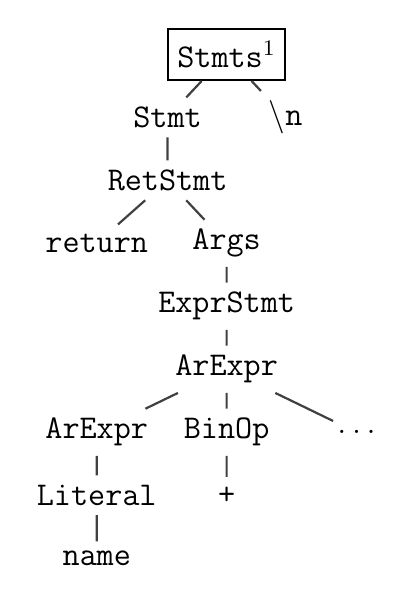
\begin{tikzpicture}
        [font=\large, edge from parent,
        % every node/.style={top color=white, bottom color=black!20,
        % ellipse, minimum size=8mm, draw=black!75,
        % thick, drop shadow, align=center},
        edge from parent/.style={draw=black!75, thick},
        level distance=0.8cm, xscale=1.0]
        \node [style={minimum size=6.5mm, draw=black, thick}] (stmts2) {\texttt{Stmts$^1$}}
        child {
            node (stmt2) {\texttt{Stmt}}
            child {
                node (RetStmt) {\texttt{RetStmt}}
                child [xscale=1.2] {
                    node (return) {\texttt{\bfseries return}}
                }
                child {
                    node (args) {\texttt{Args}}
                    child {
                        node (expr2) {\texttt{ExprStmt}}
                        child [xscale=1.1] {
                            node (arexpr1) {\texttt{ArExpr}}
                            child {
                                node (arexpr2) {\texttt{ArExpr}}
                                child {
                                    node (literal) {\texttt{Literal}}
                                    child {
                                        node (name3) {\texttt{name}}
                                    }
                                }
                            }
                            child {
                                node (binop) {\texttt{BinOp}}
                                child {
                                    node (plus) {\texttt{\bfseries +}}
                                }
                            }
                            child {
                                node (empty) {\texttt{$\dots$}}
                            }
                        }
                    }
                }
            }
        }
        child {
            node (newline3) {\texttt{\textbackslash n}}
        };
        \end{tikzpicture}
        } \subcaption{The partial parse tree for the example at
        \autoref{fig:bad-prog}.}
        \label{fig:partial-parse-tree-2}
    \end{minipage}
    \hspace{0.02\linewidth}%
    \begin{minipage}[t]{0.35\linewidth}
        \centering
        \hspace*{0.04\linewidth}%
        \resizebox{!}{0.25\textheight}{
            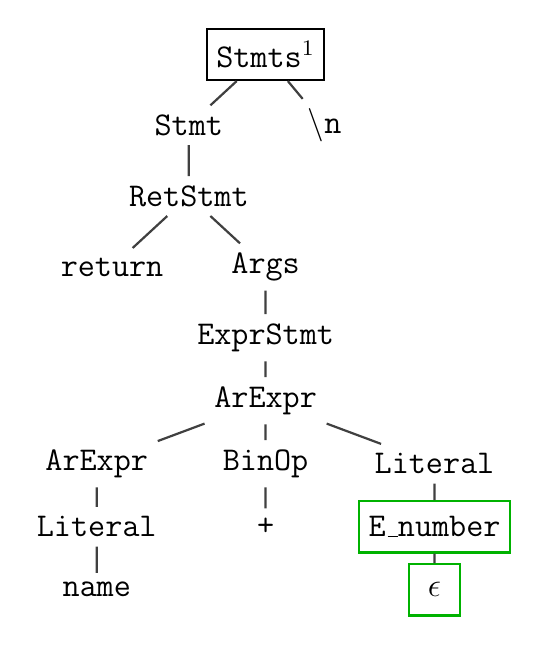
\begin{tikzpicture}
            [font=\large, edge from parent,
            % every node/.style={top color=white, bottom color=black!20,
            % ellipse, minimum size=8mm, draw=black!75,
            % thick, drop shadow, align=center},
            edge from parent/.style={draw=black!75, thick},
            level distance=0.9cm, xscale=1.0]
            \node [style={minimum size=6.5mm, draw=black, thick}] (stmts2) {\texttt{Stmts$^1$}}
            child [xscale=1.3] {
                node (stmt2) {\texttt{Stmt}}
                child {
                    node (RetStmt) {\texttt{RetStmt}}
                    child {
                        node (return) {\texttt{\bfseries return}}
                    }
                    child {
                        node (args) {\texttt{Args}}
                        child {
                            node (expr2) {\texttt{ExprStmt}}
                            child [level distance=0.8cm, xscale=1.1] {
                                node (arexpr1) {\texttt{ArExpr}}
                                child {
                                    node (arexpr2) {\texttt{ArExpr}}
                                    child {
                                        node (literal1) {\texttt{Literal}}
                                        child {
                                            node (name3) {\texttt{name}}
                                        }
                                    }
                                }
                                child {
                                    node (binop) {\texttt{BinOp}}
                                    child {
                                        node (plus) {\texttt{\bfseries +}}
                                        }
                                }
                                child {
                                    node (literal2) {\texttt{Literal}}
                                    child {
                                        node [style={minimum size=6.5mm, draw=black!30!green, thick}] (enumber) {\texttt{E\_number}}
                                        child {
                                            node [style={minimum size=6.5mm, draw=black!30!green, thick}] (eps) {\texttt{$\epsilon$}}
                                        }
                                    }
                                }
                            }
                        }
                    }
                }
            }
            child {
                node (newline3) {\texttt{\textbackslash n}}
            };
            \end{tikzpicture}
        } \subcaption{Adding a number with the green \texttt{E\_number} error rule.}
        \label{fig:adding-partial}
    \end{minipage}
    \hspace{0.01\linewidth}%
    \begin{minipage}[t]{0.32\linewidth}
        \centering
        \resizebox{!}{0.25\textheight}{
            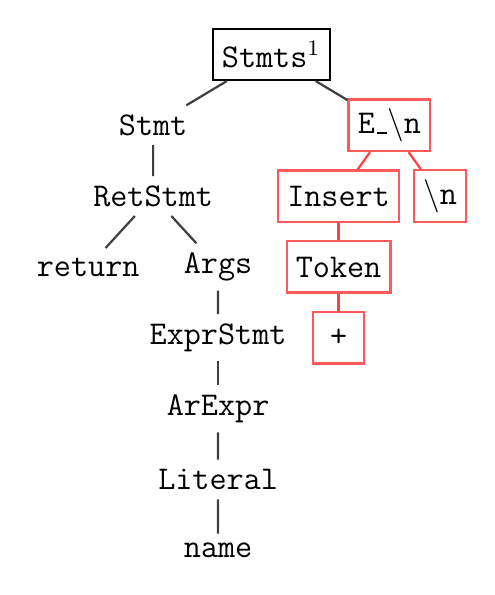
\begin{tikzpicture}
            [font=\large, edge from parent,
            % every node/.style={top color=white, bottom color=black!20,
            % ellipse, minimum size=8mm, draw=black!75,
            % thick, drop shadow, align=center},
            edge from parent/.style={draw=black!75, thick},
            level distance=0.9cm, xscale=2.0]
            \node [style={minimum size=6.5mm, draw=black, thick}] (stmts2) {\texttt{Stmts$^1$}}
            child {
                node (stmt2) {\texttt{Stmt}}
                child [xscale=0.55] {
                    node (RetStmt) {\texttt{RetStmt}}
                    child {
                        node (return) {\texttt{\bfseries return}}
                    }
                    child {
                        node (args) {\texttt{Args}}
                        child {
                            node (expr2) {\texttt{ExprStmt}}
                            child {
                            node (arexpr1) {\texttt{ArExpr}}
                                child {
                                    node (literal1) {\texttt{Literal}}
                                    child {
                                        node (name3) {\texttt{name}}
                                    }
                                }
                            }
                        }
                    }
                }
            }
            child {
                node [style={minimum size=6.5mm, draw=red!65, thick}] (enewline) {\texttt{E\_\textbackslash n}}
                child [edge from parent/.style={draw=red!75, thick}, xscale=0.43] {
                    node [style={minimum size=6.5mm, draw=red!65, thick}] (insert) {\texttt{Insert}}
                    child {
                        node [style={minimum size=6.5mm, draw=red!65, thick}] (token) {\texttt{Token}}
                        child {
                            node [style={minimum size=6.5mm, draw=red!65, thick}] (plus) {\texttt{\bfseries +}}
                        }
                    }
                }
                child [edge from parent/.style={draw=red!75, thick}, xscale=0.43] {
                    node [style={minimum size=6.5mm, draw=red!65, thick}] (newline3) {\texttt{\textbackslash n}}
                }
            };
            \end{tikzpicture}
        }
        \subcaption{Deleting the \texttt{+} with red \texttt{E\_\textbackslash n} error rule.}
        \label{fig:deleting-partial}
    \end{minipage}
    \caption{The rest of the problematic function in
    \autoref{fig:partial-parse-tree-1} and two possible error-correcting parses}
    \label{fig:two-partial-parses}
\end{figure}




% This eliminates backtracking and prevents a combinatorial explosion. Worst
% case, it has a time complexity of $O(n^3 G^2)$ for generic context-free
% grammars, where $n$ is the number of \emph{tokens} of the input program and
% $G$ is the grammar size, \ie the number of \emph{production rules} it
% includes.

% Therefore, the new and larger error correcting grammar $G'$ is introduced that
% is at least 3 times larger than $G$, making ECE-Parser not scalable for large
% programs or programs with a lot of parse errors.

\mypara{ECE Parsing Considerations for Python}
%
Unfortunately, we run into various problems if we
try to directly use an ECE-Parser for large, real-world
languages like Python.
%
\autoref{fig:partial-parse-tree-2} presents a \emph{partial
parse} of the problematic statements |Stmts|$^1$ of
\autoref{fig:partial-parse-tree-1}.
%
Considering a deletion error, the
%
|E_number $\rightarrow$ $\epsilon$| error rule is used to match the empty symbol
and generate a parse that suggests that a \emph{number} is missing after the |+|
operator. On the other hand, the
%
|E_\n $\rightarrow$ Insert \n| error rule can be used to consider a insertion
error before the new line character, basically \emph{deleting} the |+| operator.
In this case, |ArExpr $\rightarrow$ Literal| is used to parse the program
instead of |ArExpr $\rightarrow$ ArExpr BinOp Literal|.

The ECE-Parser is an effective approach on finding minimum distance parses for
programs than do not belong in the given programming language, \ie have parse
errors. However, this parsing algorithm has limited use in large real-world
programming languages, \eg Python or Java, and more time- and memory-efficient
parsing algorithms are often used, \eg LR parsing \etc \citep{Knuth_1965,
Chapman_1987}. For example, Python has \emph{$91$ terminal symbols} (including
the program's |end_marker|) which means that for all the cases of the error
rules |E_t| (excluding the non-error base case |E_t $\rightarrow$ t|), |Replace|
and |Token|, \emph{$455$ terminal error rules} have to be added to the grammar
$G'$. The Python grammar that we used has also \emph{$283$ production rules},
from which \emph{$182$ rules} have terminals in them, meaning another
\emph{$182$ error rules} need to be added. Accounting the four helper production
rules, \eg for the new start symbol, the new grammar $G'$ has \emph{$641$ new
error production rules}. This large amount of error rules renders the ECE-Parser
not scalable for large programs or programs with a lot of parse errors when
using real-world programming languages.

One of our insights,
as seen in our running example in \autoref{fig:two-partial-parses}, is that only
a handful of error rules are relevant to each parse error. Therefore, we
propose to improve ECE-Parsing's scalability by only adding \emph{a
small set} of error production rules, \ie keeping the size of $G'$ limited and
only slightly larger than the original grammar $G$. We propose to do so by
\emph{training classifiers} to select a small set of error rules only relevant
to the parse error. However, the program token sequences that we can use
may have irrelevant information, \eg the |foo| function in our example in
\autoref{fig:example-prog} that does not contribute to the parse error. To
address this problem, we propose to further \emph{abstract} our program token
sequences.

\subsection{Abstracting Program Token Sequences}
\label{sec:overview:abstraction}

As shown in Figure\ref{fig:overall-approach}, our neural component
has the task of training a classifier to predict the relevant error
rules for a given ill-parsed program.

\mypara{Problem: Representing Ill-parsed Programs}
%
As the inputs are ill-parsed, the training and classification
cannot use any form of analysis that requires a syntax tree as
input \citep{Sakkas_2020, Martinez_2013, Gulwani_2018, Wang_2018}.
%
One option is to view the ill-parsed program as a
plain \emph{sequence of tokens} eliding variable
names and such, as shown in \autoref{fig:prog-seq}.
%
Unfortunately, we found such token sequences yielded inaccurate
classifiers that were confused by irrelevant trailing
context, and hence, predicted rules that were not relevant
to repair the parse error at hand.


\begin{figure}[t]
\centering
\begin{minipage}[t]{0.56\linewidth}
\centering
\begin{ecode}
def name(name): \n
indent return name + number \n
dedent \n

def name(name): \n
indent name = name(name) + number \n
return name + \n
dedent end_marker
\end{ecode}
\subcaption{The token sequence generated by the lexer for the program.}
\label{fig:prog-seq}
\end{minipage}%
\hspace{0.02\linewidth}%
\begin{minipage}[t]{0.42\linewidth}
\centering
\begin{ecode}
Stmt \n

def name Params: \n
indent Stmt \n
return Expr BinOp \n
dedent end_marker
\end{ecode}
\subcaption{The abstracted token sequence for the same program.}
\label{fig:abstract-prog-seq}
\end{minipage}
\caption{The token sequences for the Python program example in \autoref{fig:example-prog}.}
\end{figure}

\mypara{Solution: Abstract with Partial Parses}
%
\toolname solves the problem of irrelevant context
by \emph{abstracting} the token sequences using
\emph{partial} parses parses to abstract away
the irrelevant context.
%
That is, we can use partial parse trees to represent
ill-parsed programs as \emph{abstracted token sequence}
shown in the bottom of \autoref{fig:abstract-prog-seq},
where any \emph{completed} production rules can be used
to abstract the relevant \emph{token sub-sequences}
with the high-level \emph{non-terminal}.

Figure~\ref{fig:partial-parse-tree-1} shows how partial
parses can be used to abstract long low-level
sequence of tokens into short sequences of non-terminals.
%
(1)~The function |foo| is completely parsed,
since it had no parse errors and the highest
level rule that can be used to abstract it is
%
|Stmt $\rightarrow$ FuncDef|.
%
(2)~Similarly, note that |Params $\rightarrow$ ( name )|
is another completed production rule, therefore the
low-level sequence of  parameter tokens in the |bar|
function can be abstracted to just the non-terminal |Params|.
%
(3)~However, production rule for |FuncDef|, however, is
\emph{incomplete} since the last statement |Stmt| (under |Stmts|$^1$)
has a parse error as shown in \autoref{fig:partial-parse-tree-2}.

\mypara{Problem: Ambiguity}
%
The generation of this abstraction, however,
poses another difficulty.
%
Earley parsing collects a large amount of partial
parses (via dynamic programming) until the program
is fully parsed.
%
That means at each program location, multiple
partial parses can be chosen to abstract our programs.
%
This \emph{ambiguity} can be seen even in the two
suggested repairs in \autoref{fig:two-partial-parses}:
if we delete the colored nodes in \autoref{fig:adding-partial} and
\autoref{fig:deleting-partial} we obtain two possible partial parses for our
program, the first one matching \autoref{fig:partial-parse-tree-2} and the
second one not shown here.

\mypara{Solution: Probabilistic Context-Free Grammars}
%
\toolname solves the ambiguity problem
of choosing between multiple possible
partial parses via a data-driven approach
based on \emph{Probabilistic Context-Free Grammars}
which have been used in previous work
to select \emph{complete} parses for
ambiguous grammars \citep{Collins_2013, Jelinek_1992}.
%
A PCFG associates each of its production rules with a
\emph{weight} or \emph{probability}.
%
These weights can be learned \citep{Collins_2013}
by using the data set to count the production rules
used to parse a number of programs belonging to that
language.
%
\toolname uses PCFGs to resolve the ambiguity of
partial parses by associating each partial tree
(in the Earley table) with a probability which
is the \emph{product} of the used rules' probabilities.
%
The tree with the highest probability is selected
as a final parse tree which can then be used to
generate an abstracted token sequence, as described above.


\autoref{fig:weighted-production-rules} shows the
learned probabilities for the example Python grammar.
%
We observe, for example, that |ReturnStmt| has two
possible production rules and almost $98.4\%$ of the
times a |return| is followed by an argument list.
%
Additionally, $62.6\%$ of the times a |Stmt| is an
|ExprStmt| and only $7.6\%$ of the times it is a |RetStmt|.
%
Thus, in our example, the probability that would be assigned
to the partial parse for |Stmts|$^1$ in \autoref{fig:adding-partial}
(only the sub-tree without the colored error nodes) is
the product of the probabilities of the production rules |Stmts|
$\rightarrow$ |Stmt \n|, |Stmt| $\rightarrow$ |RetStmt|, |RetStmt| $\rightarrow$
|return Args|, |Args| $\rightarrow$ |ExprStmt| \etc which is $38.77\%\ \cdot\
7.59\%\ \cdot\ 98.39\%\ \cdot\ 99.20\%\ \cdot\ \dots =
4.57\text{\textperthousand}$, while the partial parse for |Stmts|$^1$ in
\autoref{fig:deleting-partial} would similarly be calculated as
$47.61\text{\textperthousand}$, making it the proper choice for
the abstraction of the program.

\begin{figure}[t]
\begin{rules}
S        $\rightarrow$ Stmts end_marker ($p = \underline{100.0\%}$)
Stmts    $\rightarrow$ Stmt \n ($p = \underline{38.77\%}$) | Stmt \n Stmts ($p = \underline{61.23\%}$)
Stmt     $\rightarrow$ ExprStmt ($p = \underline{62.64\%}$) | RetStmt ($p = \underline{ 7.59\%}$) | ...
RetStmt  $\rightarrow$ return ($p = \underline{ 1.61\%}$) | return Args ($p = \underline{98.39\%}$)
Args     $\rightarrow$ ExprStmt ($p = \underline{99.20\%}$) | ...
ExprStmt $\rightarrow$ ArExpr ($p = \underline{29.40\%}$) | ...
ArExpr   $\rightarrow$ Literal ($p = \underline{86.89\%}$) | ArExpr BinOp Literal ($p = \underline{13.11\%}$)
Literal  $\rightarrow$ name ($p = \underline{64.89\%}$) | number ($p = \underline{20.17\%}$) | ...
\end{rules}
\caption{The production rules shown in \autoref{fig:production-rules} with
their learned \underline{probabilities}.}
\label{fig:weighted-production-rules}
\end{figure}
% S        (*@$\rightarrow$@*) Stmts end_marker        , $p = 100.0\%$
% Stmts    (*@$\rightarrow$@*) Stmt \n                 , $p = 38.77\%$
% Stmt     (*@$\rightarrow$@*) ExprStmt                , $p = 62.64\%$
% Stmt     (*@$\rightarrow$@*) RetStmt                 , $p =  7.59\%$
% RetStmt  (*@$\rightarrow$@*) return                  , $p =  1.61\%$
% RetStmt  (*@$\rightarrow$@*) return Args             , $p = 98.39\%$
% Args     (*@$\rightarrow$@*) ExprStmt                , $p = 99.20\%$
% ExprStmt (*@$\rightarrow$@*) ArExpr                  , $p = 29.40\%$
% ArExpr   (*@$\rightarrow$@*) Literal                 , $p = 86.89\%$
% ArExpr   (*@$\rightarrow$@*) ArExpr BinOp Literal    , $p = 13.11\%$
% Literal  (*@$\rightarrow$@*) name                    , $p = 64.89\%$
% Literal  (*@$\rightarrow$@*) number                  , $p = 20.17\%$
% Stmts    (*@$\rightarrow$@*) Stmt \n Stmts           , $p = 61.23\%$
% Stmt     (*@$\rightarrow$@*) FuncDef                 , $p =  7.86\%$
% Stmt     (*@$\rightarrow$@*) PassStmt                , $p =  0.13\%$
% FuncDef  (*@$\rightarrow$@*) def name Params : Block , $p = 99.10\%$
% Block    (*@$\rightarrow$@*) \n indent Stmts dedent  , $p = 99.29\%$
% Args     (*@$\rightarrow$@*) ExprStmt , Args         , $p =  0.80\%$

\subsection{Training Sequence Classifiers}
\label{sec:overview:train}

The abstracted token sequences we extracted from
the partial parses present us with short abstracted
sequences that abstract irrelevant details of the context
into non-terminals.
%
Next, \toolname uses the NLP technique of
\emph{sequence models} \citep{Sutskever_2014, Hardalov_2018}
to (use the abstract token sequences) to train
a classifier that can predict the relevant EC rules.

\mypara{Seq2Seq Architectures}
%
Sequence-to-sequence (seq2seq) architectures
transform an input sequence of tokens into a
new sequence \citep{Sutskever_2014} and consist
of an \emph{encoder} and a \emph{decoder}.
%
The encoder transforms the input token sequence
into a \emph{abstract vector} that captures all
the essence and context of the input sequence.
%
This vector does not necessarily have a physical
meaning and is instead an internal representation
of the input sequence into a higher dimensional space.
The abstract vector is given as an input to the decoder,
which in turn transforms it into an output sequence.

% Both the encoder and the decoder can be an (older) Long-Short-Term-Memory
% (LSTM)-based model \citep{Hochreiter_1997} or a more modern and state-of-the-art
% \emph{Transformer} \citep{Vaswani_2017}.

\toolname uses a \emph{Transformer classifier}
that can correctly predict a small set of relevant
error production rules for a given abstracted token sequence.
We use an \emph{transformer encoder} to encode
the input sequences into abstract vectors that
we then feed into a \emph{\dnn} classifier to
train and make accurate predictions \citep{Schmidhuber_2015}.

\mypara{Training From a Dataset}
%
Given a dataset of fixed parse errors,
such as \autoref{fig:example-prog}, we
extract the small set of relevant error
rules needed for each program to make it parse
with an ECE-Parser.
%
Running the ECE-Parser on every program
in the dataset with the \emph{full set}
of error production rules is prohibitively
slow.
%
Therefore, we extract the erroneous and
fixed program token-level differences or
\emph{token diffs} and map them to
\emph{terminal error production rules}.
%
The non-terminal error rules can be
inferred using the grammar and the terminal
rules. Next, we run the ECE-Parser with
the extracted error rules to confirm which
ones would make the program parse and assign them as
\emph{labels}.

For example, the diff for the program pair in
\autoref{fig:example-prog} would show the
deleted |+| operator, thus extracting
the error rules |Token $\rightarrow$ +|
and |E_\n $\rightarrow$ Insert \n|,
since the extra token |+| precedes
a newline character |\n|.
%
Similarly, if a token |t| is added in
the fixed program, the error rule
%
|E_t $\rightarrow$ $\epsilon$| is
added and if a token |t| replaces
a token |a| in the fix the error
rules |E_t $\rightarrow$ Replace| and
%
|Replace $\rightarrow$ a| are added.

\subsection{Predicting Error Rules with Sequence Classifiers}
\label{sec:overview:seq-classifiers}

The learned sequence classifier model,
which has be trained on the updated
error-rule-labeled data set can now
be used to predict the relevant rules
for new erroneous programs.
%
Additionally, neural networks have
the advantage of associating each
class with a \emph{confidence score}
that can be used to rank error rule
predictions for new programs, letting
us select the top-$N$ ones that will
yield accurate repairs when used
with the ECE-Parser.

For our running example, in \autoref{fig:bad-prog}, we abstract the program
shown in \autoref{fig:abstract-prog-seq} and then we predict the error
production rules for it with the trained classifier. We rank the full set of
\emph{terminal} error rules based on their predicted error score from the
classifier and return the \emph{top 10} predictions for our example. Therefore,
the predicted set of error rules is the following:
%
|E_number $\rightarrow$ $\epsilon$|, \linebreak
%
|E_number $\rightarrow$ Insert number|, |E_\n $\rightarrow$ Insert \n|,
%
|E_($\rightarrow$ $\epsilon$|,
%
|E_return $\rightarrow$ $\epsilon$|, |Token $\rightarrow$ )|,
%
|Token $\rightarrow$ +|, |Token $\rightarrow$ :|, |Token $\rightarrow$ name|,
%
|Token $\rightarrow$ number|.

The classifier predicts mostly relevant error rules such as the ones that use
|E_number|, \linebreak
%
|E_\n| and |E_return| for example, as we showed previously. There are also rules
that are not very relevant to this parse error but the classifier predicts
probably due to them being common parse errors, \eg
%
|Token $\rightarrow$ )|, |Token $\rightarrow$ :|. Finally, we added the
\emph{non-terminal} error rules needed to introduce these errors, which can be
inferred by them. For example, we can infer
%
|Stmts $\rightarrow$ Stmt E_\n|, |Stmts $\rightarrow$ Stmt E_\n Stmts| and
%
\lstinline{Block $\rightarrow$ E_\n indent Stmts dedent} from |E_\n| (we don't
need \linebreak |E_indent| or |E_dedent| here since no such terminal error rules were
predicted).

We then parse the program in \autoref{fig:bad-prog} with the ECE-Parser and
these specific error rules to generate a valid parse. We observe that it takes
our implementation (as we will show later in depth) around \emph{2 seconds} to
generate a valid parse, which is also the one that leads to the actual user
repair in \autoref{fig:fixed-prog}! On the other hand, when we use a baseline
ECE-Parser with the full set of error rules it takes \emph{2 minutes and 55
seconds} to generate a valid parse, which is, additionally, not the expected
user parse, but the one presented in \autoref{fig:adding-partial}. These
examples demonstrate the effectiveness of accurately \emph{predicting error
rules using sequence classifiers, which are trained on abstracted token
sequences}.

In the next three sections, we describe in depth the specifics of our approach
by defining all the methods in \autoref{fig:api}. We start by presenting the
program abstraction (\autoref{sec:prog-abstract}) using partial parses and a
learnt PCFG, we then explain how we train sequence models for making error rule
predictions (\autoref{sec:seq-classifiers}) and, finally, we demonstrate our
algorithms for building \toolname, an approach for efficiency parsing erroneous
programs.
